\documentclass[10pt,openright,twoside,french]{book}

\input philippe2013
\input philippe2013_cours
\input philippe2013_sections
\input philippe2013_chapitre
\renewcommand\PartProgramme{Fonctions}
\renewcommand\MaCouleur{Melon!150}

\pieddepage{}{%
\begin{tikzpicture}[scale=0.65]
\shadedraw [top color=white, bottom color=\MaCouleur, draw=\MaCouleur]
[l-system={Sierpinski triangle, step=1pt, angle=60, axiom=F, order=6.5}]
lindenmayer system -- cycle;
\draw (30:0.65cm) node {\bfseries\textcolor{black}{\thepage}};
\end{tikzpicture}%
}{}

\setcounter{chapter}{1}

\begin{document}
\chapter{Suites}\label{ch_suite}

\section{Définir une suite}
\begin{Defi}
    Une \ipt{suite numérique} $u$ est une fonction de $\N$ dans $\R$. On note alors :
    \[\begin{array}{rcl}
        u\colon \N & \to & \R \\
        n & \mapsto & u(n) = u_n
    \end{array}\]
\end{Defi}\medskip

\begin{Rmq}
    Le premier terme de la suite sera alors le terme de rang (d'indice) $0$ : $u(0)$. Le suivant est le terme de rang (d'indice) $1$ : $u(1)$. Puis $u(2)$\ldots Dans le cas des suites, on notera plutôt $u_0$, $u_1$, $u_2$\ldots\par
    Pour parler d'une suite, on dira la suite $u$, ou encore la suite $(u_n)_{n \in \N}$.\par
    Pour alléger l'écriture, on pour écrire la suite $(u_n)$ mais il ne faut pas confondre avec le terme de rang $n$ qui se note $u_n$ ou $u(n)$.
\end{Rmq}

\subsection{Suite définie explicitement}

\begin{Defi}
    Une suite $(u_n)_{n\in \N}$ est définie \iptb{explicitement}\index{suite!définie explicitement} lorsque l'on connaît l'expression de $u_n$ en fonction de $n$. On peut donc calculer directement la valeur de $u_n$.
\end{Defi}

\begin{Exemple}[s]
     \begin{enumerate}
        \item On considère la suite $(u_n)$ définie pour tout $n \in \N$ par $u_n = 2n^2 - 3$.\par
        Le terme initial est $u_0 = 2 \times 0^2 - 3 = -3$. Le terme suivant est $u_1 = 2 \times 1^2 - 3 = -1$.\par
        $u_{10} = 2 \times 10^2 - 3 = 2 \times 100 - 3 = 197$.
        Le quinzième terme est $u_{14} = 2 \times 14^2 - 3 = 389$.
        \item On considère la suite $(v_n)$ définie pour tout $n \in \N^*$ par $v_n = \frac1n$.\par
        Le terme initial est $v_1 = \frac 1 1 = 1$. Le $15$\ieme terme est $v_{15} = \frac{1}{15}$.
     \end{enumerate}
\end{Exemple}

\subsection{Suite définie par récurrence}

\begin{Defi}
    Une suite $(u_n)_{n\in \N}$ est définie par \iptb{récurrence} \index{suite!définie par récurrence} lorsque l'on connaît l'expression de $u_n$ en fonction de $u_{n-1}$. Pour calculer un terme d'une suite, il faut donc connaître le précédent. Pour cela, le terme initial est généralement donné avec la définition de la suite.
\end{Defi}

\begin{Exemple}
    On considère la suite $u_n$ définie par :
    $\left\{
    \begin{array}{l}
        u_0 = \frac 13\\
        u_{n +1} = \frac 34 u_n - 1 \quad \text{pour tout $n\in \N^*$}
    \end{array}
    \right.$\par\medskip
    On a alors $u_0 = \frac 13$, $u_1 = \frac 3 4 \times u_0 - 1 = \frac34 \times \frac 13 - 1 = \frac 14 - 1 = -\frac34$.\par
    Puis $u_2 = \frac 3 4 \times u_1 - 1 = \frac34 \times \left(-\frac 34\right) - 1 = -\frac{9}{16} - 1 = -\frac{25}{16}$
\end{Exemple}

\begin{Rmq}
    Dans tous les cas, l'utilisation d'un tableur ou d'une calculatrice peut s'avérer très utile pour calculer rapidement les premiers termes d'une suite ainsi que pour les représenter graphiquement.
\end{Rmq}

\section{Suites particulières}
\subsection{Suite arithmétique}

\begin{Defi}
    Une suite $(u_n)_{n\in \N}$ est dite \iptb{arithmétique} \index{suite!arithmétique} lorsqu'il existe un nombre réel $r$ tel que, pour tout $n \in \N$, $u_{n+1} = u_n + r$.\par
    Le réel $r$ est appelé la \ipt{raison} de la suite $(u_n)$
\end{Defi}\medskip

\begin{Exemple}
    Des parents ouvrent un compte en banque pour leur enfant. Lors de l'ouverture, ils  versent \EUR{$50$} puis, au début de chaque mois, ils rajoutent \EUR{$100$}.\par
    On définit alors une suite $(c_n)_{n\in\N}$ où le terme $n$ de la suite correspond au montant présent sur le compte $n$ mois après son ouverture.\par
    On a donc $c_0 = 50$ et, pour tout $n \in \N^*$, $c_{n+1} = c_n + 100$.\par
    La suite $(c_n)$ est donc une suite arithmétique.

    \begin{center}
    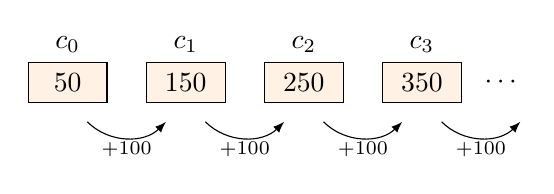
\begin{tikzpicture}[>=latex]
        \draw[fill=orange!10] (0,0) rectangle ++(1,0.5) node[midway] {\EUR{$50$}};
            \draw (0.5,0.5) node[above] {$c_0$};
        \draw[fill=orange!10] (1.5,0) rectangle ++(1,0.5) node[midway] {\EUR{$150$}};
            \draw (2,0.5) node[above] {$c_1$};
        \draw[fill=orange!10] (3,0) rectangle ++(1,0.5) node[midway] {\EUR{$250$}};
            \draw (3.5,0.5) node[above] {$c_2$};
        \draw[fill=orange!10] (4.5,0) rectangle ++(1,0.5) node[midway] {\EUR{$350$}};
            \draw (5,0.5) node[above] {$c_3$};
        \draw (6,0.25) node {$\cdots$};
        %
        \draw[->] (0.75,-0.25) to[bend right=45] ++(1,0); \draw (1.25,-0.6) node {\scriptsize\EUR{$+100$}};
        \draw[->] (2.25,-0.25) to[bend right=45] ++(1,0); \draw (2.75,-0.6) node {\scriptsize\EUR{$+100$}};
        \draw[->] (3.75,-0.25) to[bend right=45] ++(1,0); \draw (4.25,-0.6) node {\scriptsize\EUR{$+100$}};
        \draw[->] (5.25,-0.25) to[bend right=45] ++(1,0); \draw (5.75,-0.6) node {\scriptsize\EUR{$+100$}};
    \end{tikzpicture}
\end{center}
\end{Exemple}\medskip

\begin{Rmq}
    Considérons une suite arithmétique $(u_n)_{n \in \N}$, de raison $r$ et essayons de déterminer une définition explicite de cette suite. Pour tout $n \in \N^*$,
    \[u_{n} = u_{n-1} + r = u_{n-2} + r + r = u_{n-3} + r + r + r = \ldots = u_0 + r + \cdots + r = u_0 + n \times r\]
    On rappelle que $u_0$ et $r$ sont fixés et que le nombre $n$ est la variable. Donc, en employant les notations des fonctions, on obtient :
    \[u(n) = r \times n + u_0.\]
    Non seulement on a défini $(u_n)$ explicitement mais de plus, on constate qu'une suite arithmétique est une fonction affine (définie sur $\N$ uniquement) dont le \coef directeur est la raison $r$ et l'ordonnée à l'origine est $u_0$. On en déduit les résultats suivants :
\end{Rmq}\medskip

\begin{Prop}
    Une suite arithmétique est représentée graphiquement par des points alignés.
\end{Prop}\medskip

\begin{Thm}
    Une suite arithmétique de raison $r$ est :
    \begin{itemize}
        \item croissante si $r > 0$ ;
        \item décroissante si $r < 0$ ;
        \item constante si $r = 0$.
    \end{itemize}
\end{Thm}

\subsection{Suite géométrique}

\begin{Defi}
    Une suite $(u_n)_{n\in \N}$ est dite \iptb{géométrique} \index{suite!géométrique} lorsqu'il existe un nombre réel $q$ \textbf{non nul} tel que, pour tout $n \in \N$, $u_{n+1} = u_n \times q$.\par
    Le réel $q$ est appelé la \ipt{raison} de la suite $(u_n)$
\end{Defi}\medskip

\begin{Exemple}
    Un professeur décide de faire copier des lignes à chaque élève qui parlera sans autorisation. Le premier copiera $10$ lignes, le suivant $2$ fois plus, et ainsi de suite en multipliant le nombre de lignes par $2$ à chaque fois.\par
    On définit alors une suite $(\ell_n)_{n\in\N^*}$ où le terme $n$ de la suite correspond au nombre de ligne copiée par le $n$\ieme élève.\par
    On a donc $\ell_1 = 10$ et, pour tout $n \in \N^*$, $\ell_{n+1} = \ell_n \times 2$.\par
    La suite $(\ell_n)$ est donc une suite géométrique.

    \begin{center}
    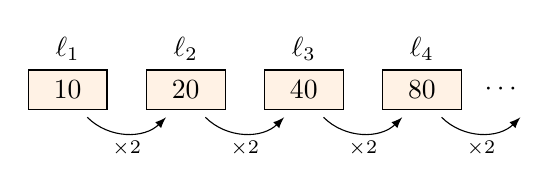
\begin{tikzpicture}[>=latex]
        \draw[fill=orange!10] (0,0) rectangle ++(1,0.5) node[midway] {$10$};
            \draw (0.5,0.5) node[above] {$\ell_1$};
        \draw[fill=orange!10] (1.5,0) rectangle ++(1,0.5) node[midway] {$20$};
            \draw (2,0.5) node[above] {$\ell_2$};
        \draw[fill=orange!10] (3,0) rectangle ++(1,0.5) node[midway] {$40$};
            \draw (3.5,0.5) node[above] {$\ell_3$};
        \draw[fill=orange!10] (4.5,0) rectangle ++(1,0.5) node[midway] {$80$};
            \draw (5,0.5) node[above] {$\ell_4$};
        \draw (6,0.25) node {$\cdots$};
        %
        \draw[->] (0.75,-0.1) to[bend right=45] ++(1,0); \draw (1.25,-0.5) node {\scriptsize$\times 2$};
        \draw[->] (2.25,-0.1) to[bend right=45] ++(1,0); \draw (2.75,-0.5) node {\scriptsize$\times 2$};
        \draw[->] (3.75,-0.1) to[bend right=45] ++(1,0); \draw (4.25,-0.5) node {\scriptsize$\times 2$};
        \draw[->] (5.25,-0.1) to[bend right=45] ++(1,0); \draw (5.75,-0.5) node {\scriptsize$\times 2$};
    \end{tikzpicture}
\end{center}
\end{Exemple}\medskip

\begin{Rmq}
    Considérons une suite géométrique $(v_n)_{n \in \N}$, de raison $q$ et essayons de déterminer une définition explicite de cette suite. Pour tout $n \in \N^*$,
    \[v_{n} = v_{n-1} \times q = v_{n-2} \times q \times q = v_{n-3} \times q \times q \times q = \ldots = v_0 \times q \times \cdots \times q = v_0 \times q^n\]
\end{Rmq}\medskip

\begin{Thm}
    On considère une suite $(u_n)_{n\in\N}$ telle que, pour tout $n \in \N, u_n > 0$.
    On suppose que $(u_n)$ est une suite géométrique de raison $q > 0$. Alors, $(u_n)$ est :
    \begin{itemize}
        \item croissante si $q > 1$ ;
        \item décroissante si $q < 1$ ;
        \item constante si $q = 1$.
    \end{itemize}
\end{Thm}

\begin{Demo}
    \begin{itemize}
        \item Lorsque $q = 1$ alors $u_0 = u_1 = u_2 =\ldots$ et la suite $u$ est constante.
        \item Sinon, pour tout $n \in \N$, on a $u_{n+1} = qu_n$. Puisque, pour tout $n \in \N$, $u_n > 0$, on peut alors écrire $\frac{u_{n+1}}{u_n} = q$. Cette fraction est strictement positive puisque c'est le quotient de deux nombres strictement positif.\par
            Depuis le collège, on sait que si $q<1$, cela signifie que le numérateur est inférieur au dénominateur. Donc, pour tout $n \in \N$, $u_{n+1} < u_n$ et la suite est donc décroissante.\par
            Si $q > 1$, cela signifie que le numérateur est supérieur au dénominateur. Donc, pour tout $n \in \N$, $u_{n+1} > u_n$ et la suite est donc croissante.
    \end{itemize}
\end{Demo}

\end{document}
